\documentclass[11pt]{article}
\usepackage{enumerate}
\usepackage{amsmath}
\usepackage{amssymb}
\usepackage{geometry}
\usepackage{graphicx}
\usepackage{amsfonts}
\usepackage{array}


\title{\Huge{Conceptos de Sistemas Operativos\\
Practica 4}}
\author{\huge{Ramiro Cabral}}
\date{\today}

\begin{document}
\maketitle
\tableofcontents
\pagebreak


\section{Procesos}
\begin{itemize}
    \item Programa en ejecucion.
    \item Segun su historial de ejecucion, podemos clasificarlos en:
        \begin{itemize}
            \item CPU bound (ligados a la CPU).
            \item I/O bound (ligados a la E/S).
        \end{itemize}
\end{itemize}

\subsection{PCB (Process Control Block)}
\begin{itemize}
    \item Una por proceso.
    \item Contiene informacion del proceso.
    \item Es lo primero que se crea cuando se realiza un fork y lo utlimo que se desaloca cuando termina.
\end{itemize}

\subsection{Tiempos de los procesos}
\begin{itemize}
    \item \textbf{Retorno:} Tiempo que transcurre entre que el proceso llega al sistema hasta que completa su ejeucion.
    \item \textbf{Espera:} Tiempo que el proceso se encuentra en el sistema esperando, es decir el tiempo que pasa sin ejecutarse. (Tiempo de retorno - Tiempo de CPU)
    \item \textbf{Promedios:} Tiempos promedio de los anteriores.
\end{itemize}

\section{Schedulers/Planificadores}
\begin{itemize}
    \item Es la clave de la multiprogramacion.
    \item Esta diseñado para cumplir con los siguientes objetivos:
        \begin{itemize}
            \item Menor tiempo de respuesta.
            \item Mayor rendimiento.
            \item Uso eficiente del procesador.
        \end{itemize}
\end{itemize}

\subsection{Tipos de Schedulers}
\begin{itemize}
    \item \textbf{Long term scheduler:} Admite nuevos procesos a memoria (controla el grado de multipfogramacion).
    \item \textbf{Medium term scheduler:} Realiza el swapping (intercambio) entre el disco y la memoria cuando el SO lo determina.
    \item \textbf{Short term scheduler:} Determina que proceso pasara a ejecutarse.
\end{itemize}

\begin{align}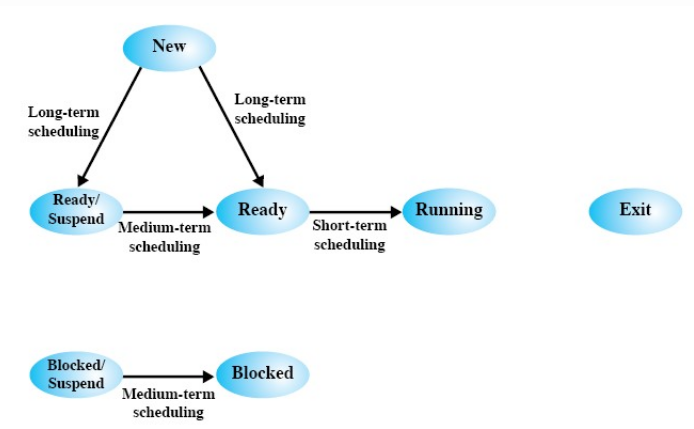
\includegraphics[width=0.8\linewidth]{assets/b.png}\end{align}
\begin{align}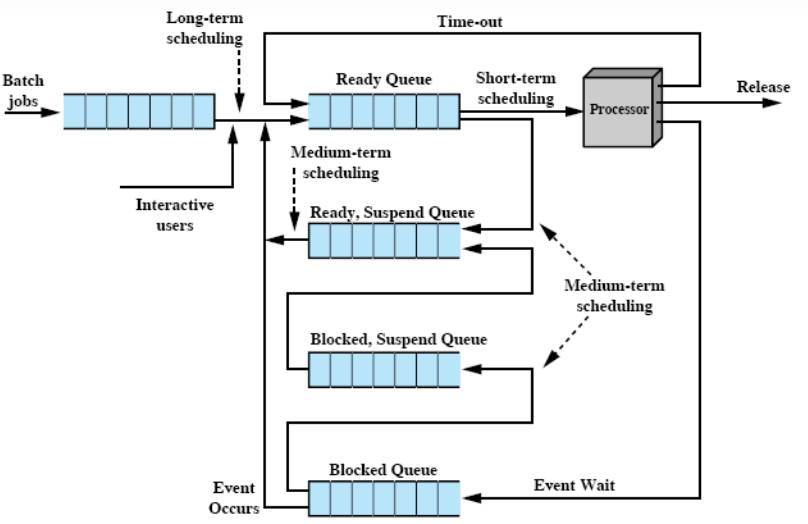
\includegraphics[width=0.8\linewidth]{assets/asd.png}\end{align}

\subsection{Apropiacion vs No apropiacion}
\begin{itemize}
    \item \textbf{Nonpreemptive:} Una vez que un proceso esta en estado de ejecucion, continua hasta que termina o se bloquea por algun evento (por ejemplo, I/O).
    \item \textbf{Preemptive:} El proceso en ejecucion puede ser interrumpido y llevado a la cola de ready
        \begin{itemize}
            \item Mayor overhead pero mejor servicio.
            \item Un proceso no monopoliza el procesador.
        \end{itemize}
\end{itemize}

\section{Algoritmos de planificacion}

\subsection{FCFS (First Come First Served)}
\begin{itemize}
    \item \textbf{Nonpreemptive}.
    \item Cuando hay que elegir un proceso para ejecutar, se selecciona el mas viejo.
    \item No favorece a ningun tipo de procesos, pero en principio podriamos decir que los CPU Bound terminan al comenzar su primer rafaga, mientras que los I/O Bound no.
\end{itemize}

\subsection{SJF (Shortest Job First)}
\begin{itemize}
    \item \textbf{Nonpreemptive}.
    \item Politica que selecciona el proceso con la rafaga de CPU mas corta.
    \item Calculo basado en la ejecucion previa.
    \item Procesos cortos se colocan delante de procesos largos.
    \item Los procesos largos pueden sufrir starvation.
\end{itemize}

\subsection{SRTF (Shortest Remaining Time First)}
\begin{itemize}
    \item Version \textbf{preemptive} de SJF.
    \item Selecciona el proceso al cual le resta menos tiempo de ejecucion en su siguiente rafaga.
    \item Favorece al los procesos I/O Bound.
\end{itemize}

\subsection{RR (Round Robin)}
\begin{itemize}
    \item Politica basada en un reloj.
    \item \textbf{Quantum (Q)} : medida que determina cuanto tiempo podra usar el procesador cada proceso:
    \item Cuando un proceso es expulsado de la CPU es colocado al final de la Ready Queue y se selecciona otro (FIFO circular).
    \item Existe un contador que indica las unidades de CPU en las que el proceso se ejecuto. Cuando el mismo llega a 0 el proceso es expulsado.
    \item El contador puede ser global o local (PCB de cada proceso).
    \item Existen dos variantes con respecto al valor inicial del contador cuano un proceso es asignado a la CPU:
        \begin{itemize}
            \item Timer Variable.
            \item Timer Fijo.
        \end{itemize}
\end{itemize}

\subsubsection{Timer Variable}
\begin{itemize}
    \item El contador se inicializa en Q cada vez que un proceso es asignado a la CPU.
    \item Es el mas utilizado.
\end{itemize}

\subsubsection{Timer Fijo}
\begin{itemize}
    \item El contador se inicializa en Q cuando su valor es cero
    \item Se puede ver como un valor de Q compartido entre los procesos.
\end{itemize}

\subsection{Prioridades}
\begin{itemize}
    \item Cada proceso tiene un valor que representa su prioridad.
    \item Se seleccina el proceso de mayor prioridad de los que se encuentran en la Ready Queue.
    \item Existe una Ready Queue para cada nivel de prioridad.
    \item Procesos de baja prioridad pueden sufrir starvation.
        \begin{itemize}
            \item Solucion: permitir a un proceso cambiar su prioridad durante su ciclo de vida (\textbf{Aging o Penalty}).
        \end{itemize}
    \item Puede ser un algoritmo \textit{preemptive} o no.
\end{itemize}


\subsection{CPU + I/O}
\begin{itemize}
    \item Ciclo de vida de un proceso: uso de CPU + operaciones de I/O.
    \item Cada dispositivo tiene su cola de procesos en espera, un scheduler por cada cola.
    \item Se considera I/O independiente de la CPU (DMA, PCI, etc). Tenemos uso de CPU y operaciones de I/O en simultaneo.
\end{itemize}

\subsection{Criterios de desempate}
\begin{enumerate}
    \item Orden de llegada de los procesos.
    \item \textbf{PID} de los procesos(el de menor PID se ejecuta primero).
\end{enumerate}


\section{Colas Multinivel}
\begin{itemize}
    \item La ready queue es dividida en varias colas (similar a prioridades).
    \item Los procesos se colocan en las colas segun una clasificacion que realice el sistema operativo.
    \item Cada cola posee su propio algoritmo de planificacion (\textbf{planificador horizontal}).
    \item A su vez existe un algoritmo que planifica las colas (\textbf{planificador vertical}).
    \item \textbf{Retroalimentacion:} un proceso puede cambiar de una cola a otra.
\end{itemize}


\section{Planificacion con multiples procesadores.}
\begin{itemize}
    \item \textbf{Planificacion temporal}: que proceso y durante cuanto.
    \item \textbf{Planificacion espacial}: en que procesador ejecutar:
    \begin{itemize}
        \item \textbf{Huella:} estado que el proceso va dejando en la cache de un procesador.
        \item \textbf{Afinidad:} preferencia de un proceso para ejecutar en un procesador.
    \end{itemize}
    \item La asignacion de procesos a un procesador puede ser:
        \begin{itemize}
            \item \textbf{Estatica:} existe una afinidad de un proceso a una CPU.
            \item \textbf{Dinamica:} la carga se comparte, se da un balancdeo de carga.
        \end{itemize}
    \item La politica puede ser:
        \begin{itemize}
            \item \textbf{Tiempo compartido:} se puede considerar una cola global o una cola local a cada procesador.
            \item \textbf{Espacio compartido:} 
                \begin{itemize}
                    \item \textbf{Grupos (threads).}
                    \item \textbf{Particiones.}
                \end{itemize}
        \end{itemize}
\end{itemize}


\subsection{Clasificaciones}
\begin{itemize}
    \item \textbf{Procesadores homogeneos:} todas las CPUs son iguales. No existe ventajas fisicas sobre el resto.
    \item \textbf{Procesadores heterogeneos:} cada procesador tiene su propia cola, su propio clock y su propio algoritmo de planificacion.
\end{itemize}

\subsection{Otra clasificacion:}
\begin{itemize}
    \item \textbf{Procesadores debilmente acoplados:} cada CPU tiene su propia memoria principal y canales.
    \item \textbf{Procesadores fuertemente acoplados:} comparten memoria y canales.
    \item \textbf{Procesadores especializados:} uno o mas procesadores principales de uso general y uno o mas procesadores de uso especifico.
\end{itemize}
\end{document}
